\section*{Methodology}

\subsection*{PyKEEN}

\todo{FURTHER EXPLAIN MODELS USED IN EXPERIMENTATION}

PyKEEN \cite{pykeen} is an open-source Python library that facilitates training and evaluation of knowledge graph embedding models. It streamlines the process of embedding entities and relations into continuous vector spaces, enabling efficient link prediction and relationship classification.

\todo{COULD USE HYPERPARAMETER TUNING: INCREASE EPOCHS}

In this project, PyKEEN was used to predict missing links within a knowledge graph through a structured workflow involving data extraction, preparation, model training, and link prediction. Triples $(h, r, t)$ representing head entities, relationships, and tail entities were first retrieved from the Neo4j database using Cypher queries (Listing~\ref{lst:cypher_query}). These triples were then converted into PyKEEN's \texttt{TriplesFactory} format to enable seamless integration with the PyKEEN pipeline. The RotatE algorithm was employed to train the embedding model over $20$ epochs with an embedding dimension of $128$. It's worth noting that $20$ epochs may be insufficient for meaningful training on large or complex graphs, especially with a high embedding dimensionality. Additionally, applying early stopping in this scenario is unlikely to yield significant improvements due to the limited number of epochs.

Finally, the trained model was used to perform link prediction, identifying potential relationships within the knowledge graph.

\begin{lstlisting}[caption=Cypher query to retrieve triples., label=lst:cypher_query]
MATCH (h)-[r]->(t)
RETURN id(h) AS head, type(r) AS relation, id(t) AS tail
\end{lstlisting}

\subsection*{Neo4j Desktop}

Neo4j Desktop \cite{neo4j} serves as a crucial tool for managing and querying the knowledge graph used in this project. It provides a local environment to import, visualize, and manipulate graph data, facilitating seamless interaction with the dataset. Neo4j's support for Cypher, its declarative graph query language, enables efficient extraction of triples representing relationships between entities. This functionality is essential for preparing the knowledge graph data, which is subsequently processed using PyKEEN for link prediction and multi-class relationship classification. By leveraging Neo4j Desktop, we ensure that the data pipeline from graph ingestion to embedding model training remains streamlined and adaptable.

\subsubsection*{Setup and Database Import}

This section provides a step-by-step guide to set up Neo4j Desktop and import a database dump file, as depicted in Figure~\ref{fig:neo4j-setup}. The specific dump used in this midterm report, derived from Hetionet, requires DBMS version $4.3$ to ensure compatibility.

\begin{figure}[ht]
    \centering
    \begin{subfigure}[b]{0.49\textwidth}
        \centering
        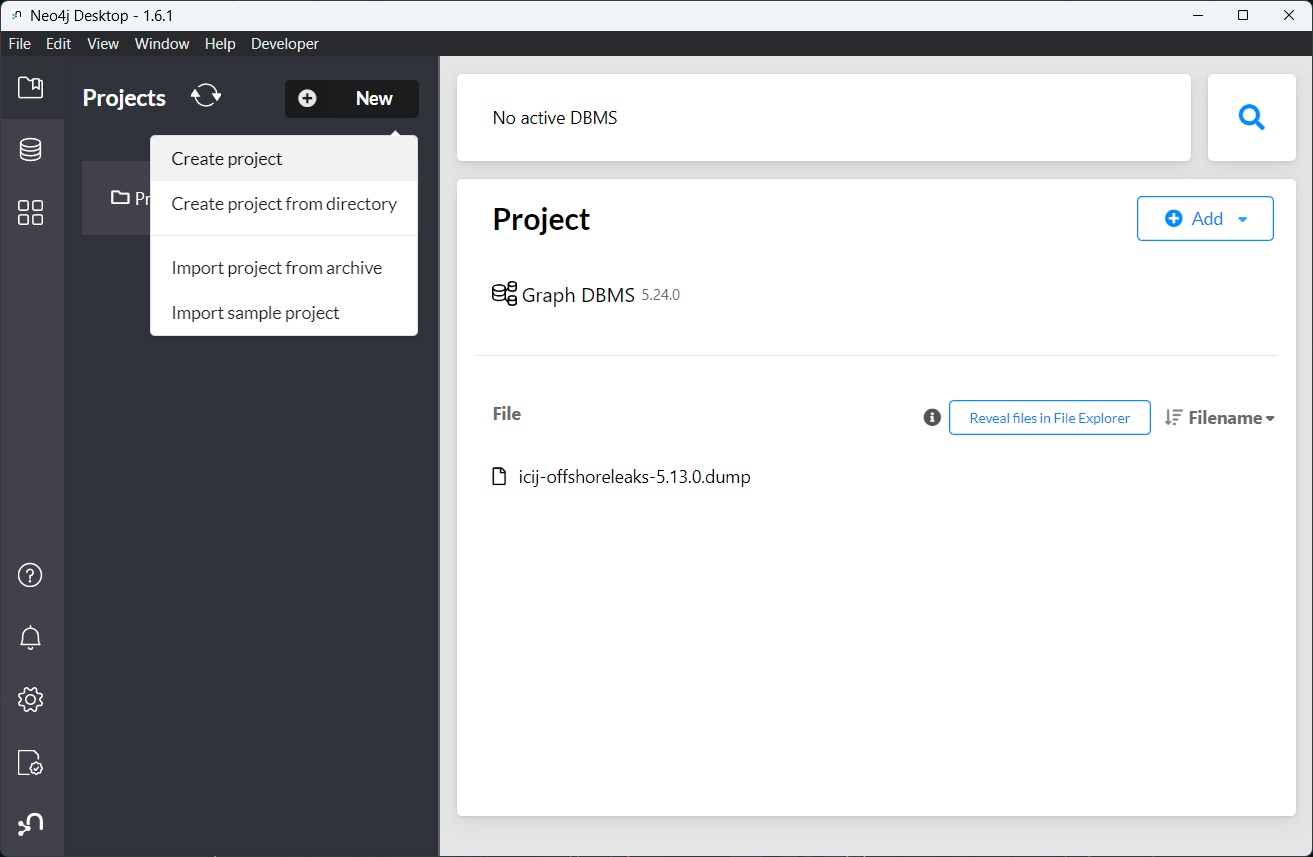
\includegraphics[width=\textwidth]{images/neo4j-setup/1}
        \caption{Creating a project.}
    \end{subfigure}
    \hfill
    \begin{subfigure}[b]{0.49\textwidth}
        \centering
        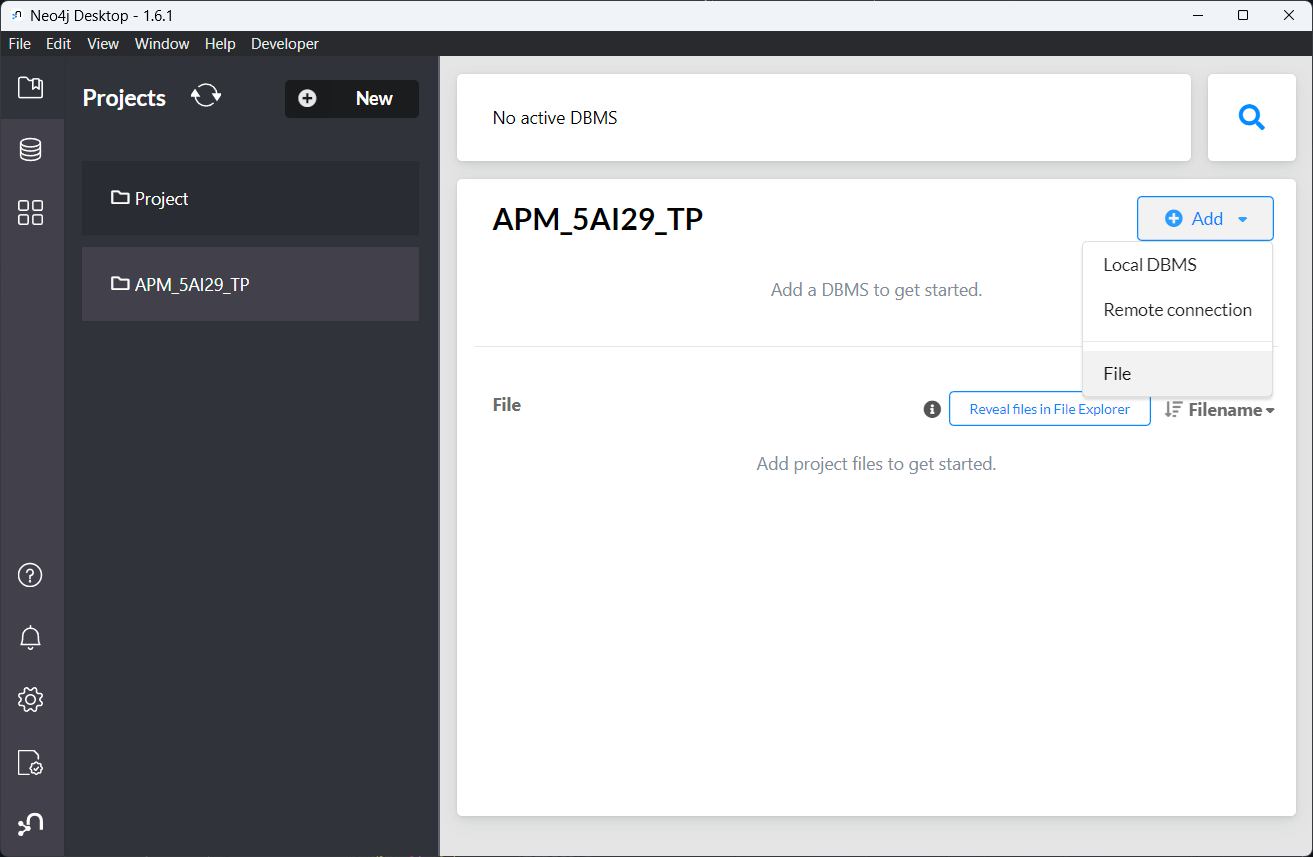
\includegraphics[width=\textwidth]{images/neo4j-setup/2}
        \caption{Adding dump file.}
    \end{subfigure}
    \\
    \begin{subfigure}[b]{0.49\textwidth}
        \centering
        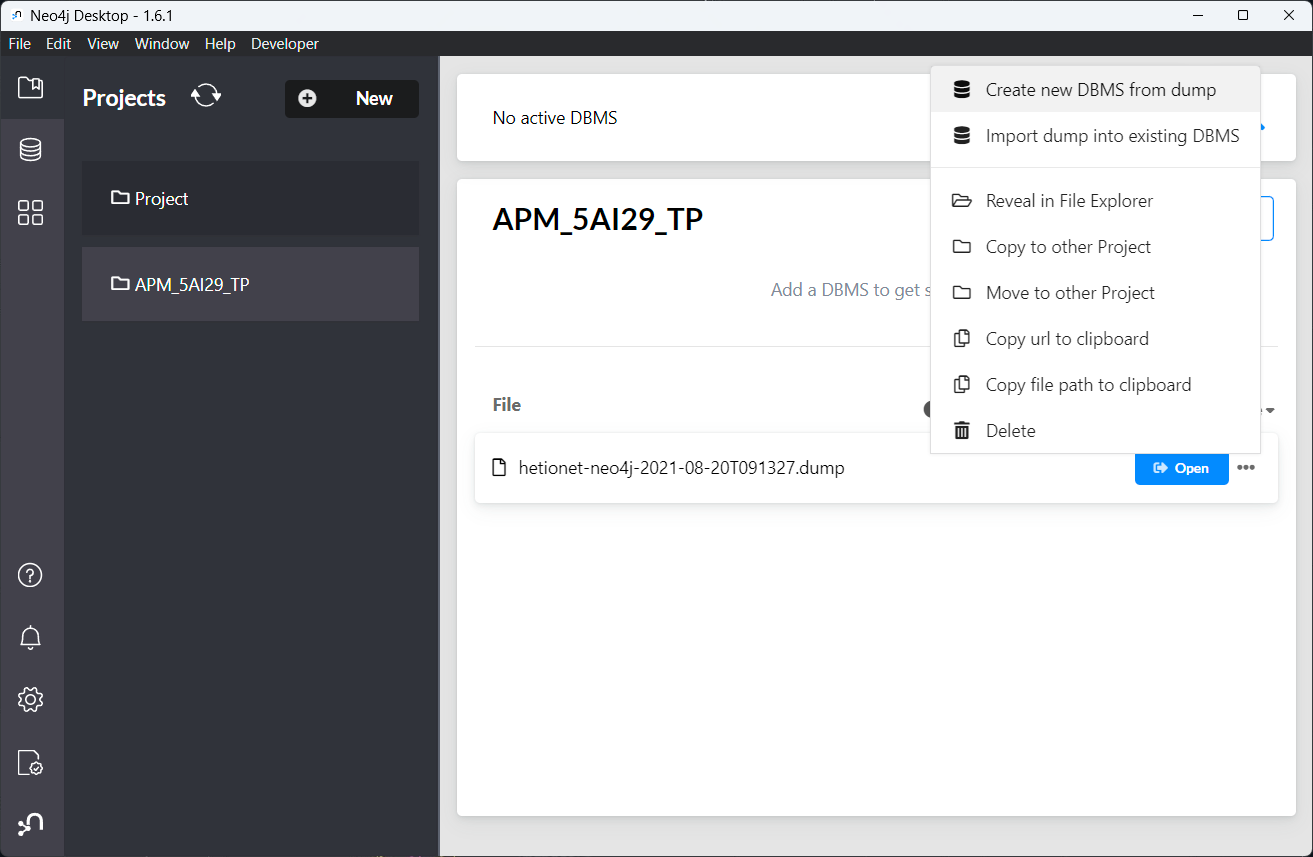
\includegraphics[width=\textwidth]{images/neo4j-setup/3}
        \caption{Importing dump to DBMS.}
    \end{subfigure}
    \hfill
    \begin{subfigure}[b]{0.49\textwidth}
        \centering
        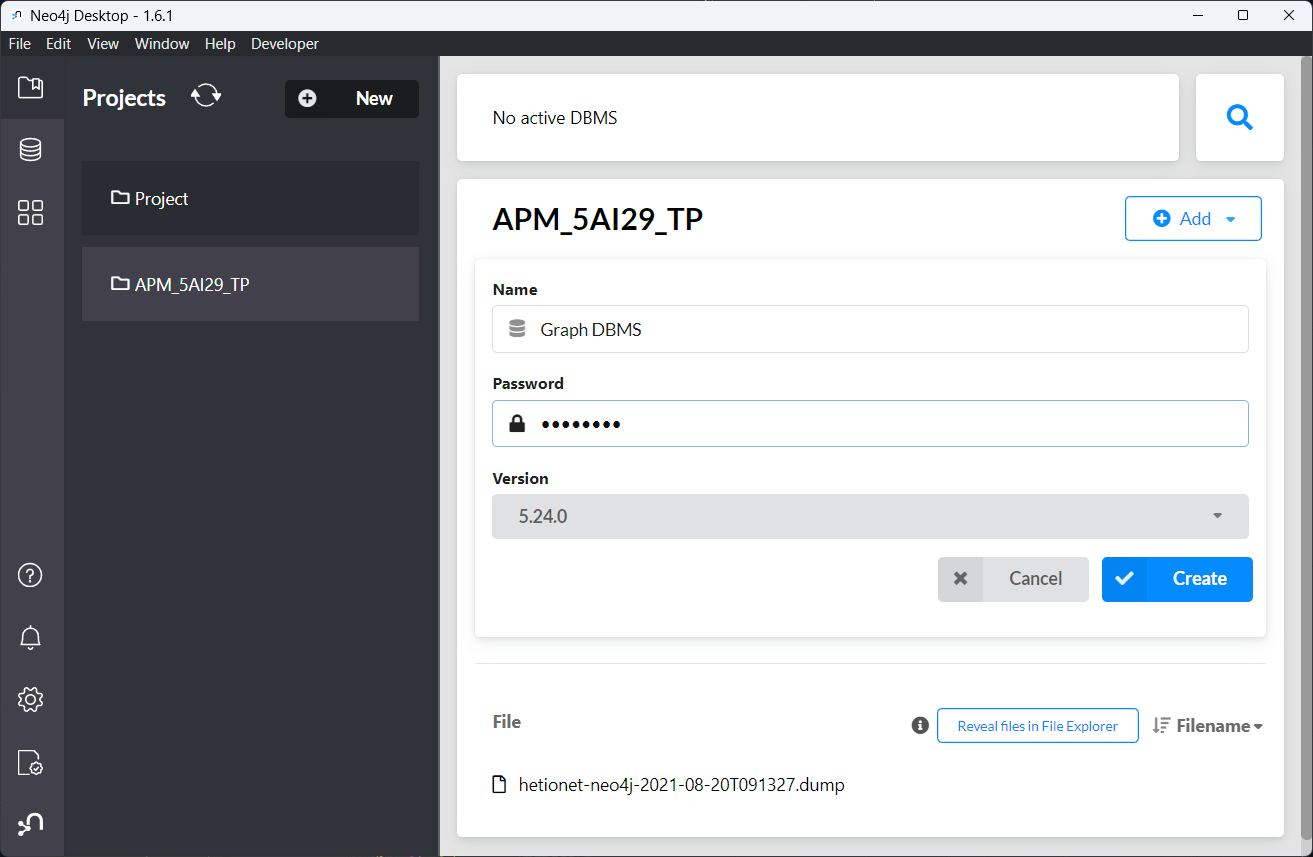
\includegraphics[width=\textwidth]{images/neo4j-setup/4}
        \caption{Configuring DBMS.}
    \end{subfigure}
    \\
    \begin{subfigure}[b]{0.49\textwidth}
        \centering
        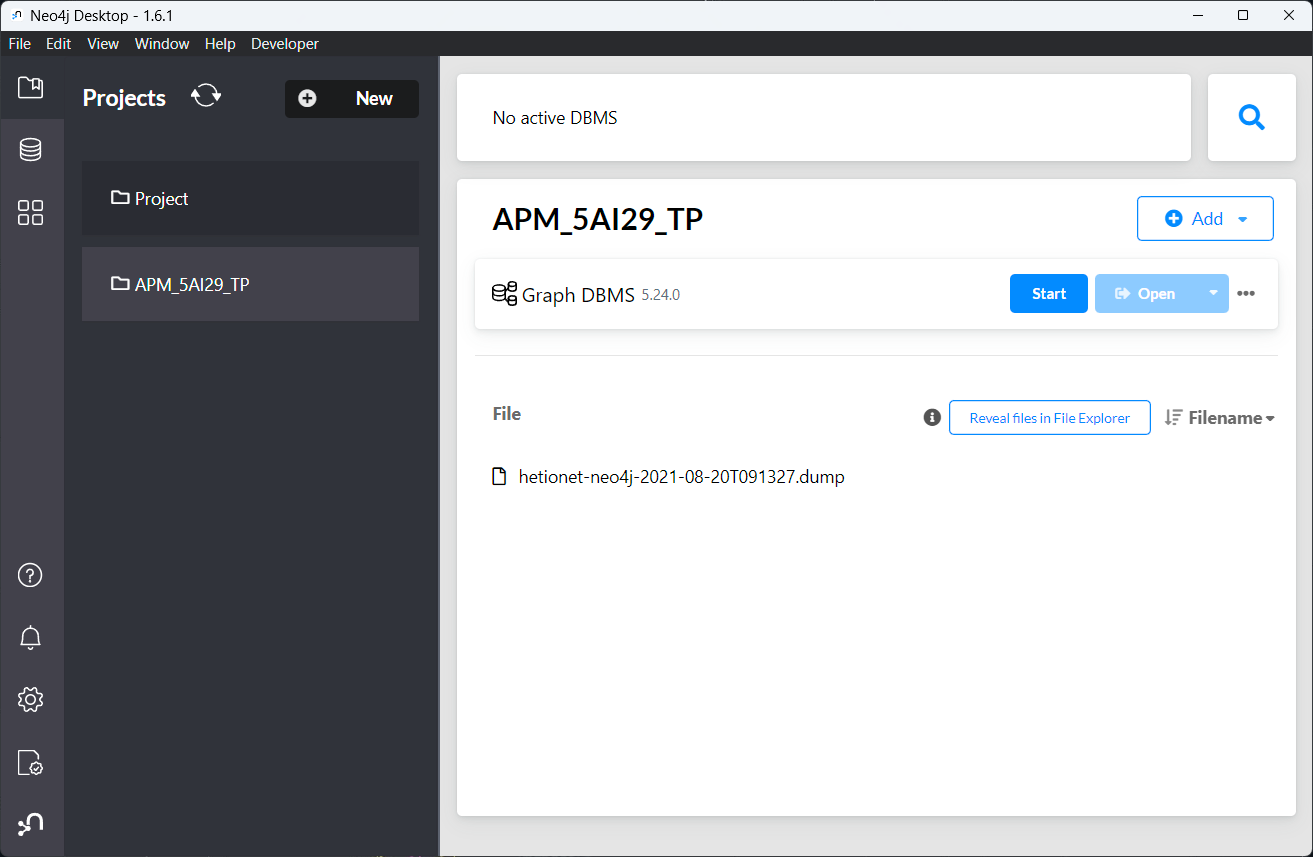
\includegraphics[width=\textwidth]{images/neo4j-setup/5}
        \caption{Starting DBMS.}
    \end{subfigure}
    \hfill
    \begin{subfigure}[b]{0.49\textwidth}
        \centering
        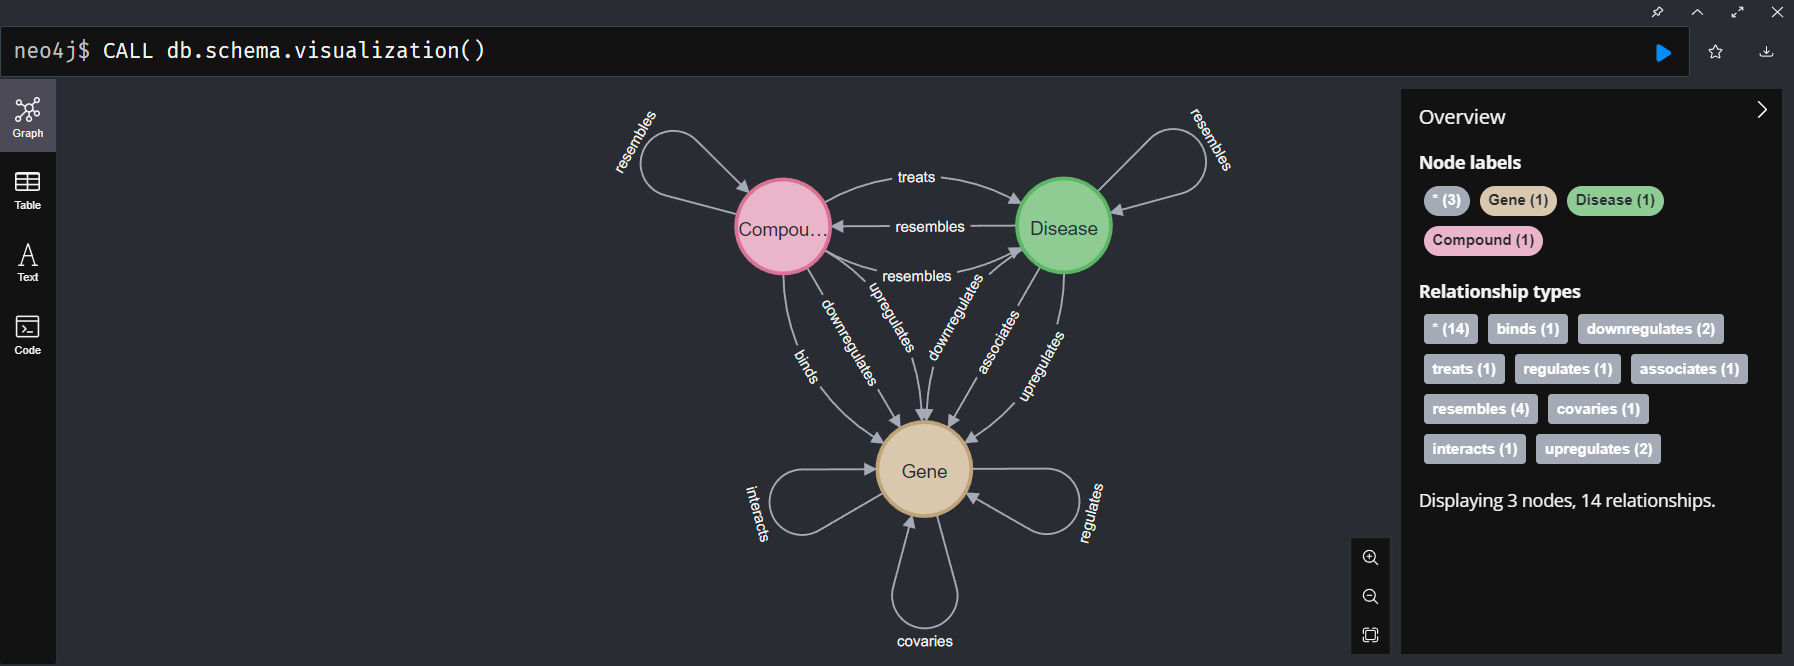
\includegraphics[width=\textwidth]{images/neo4j-setup/7}
        \caption{Visualizing schema.}
    \end{subfigure}

    \caption{Steps for Neo4j Desktop Setup.}
    \label{fig:neo4j-setup}
\end{figure}

Upon successful import, the schema can be visualized using the following Neo4j query: \texttt{CALL db.schema.visualization()}. The resulting graph, illustrates key entities and relationships that form the basis for multi-class link prediction and knowledge graph completion in subsequent tasks.

\subsection*{Large Language Models}

\todo{SOMEONE STILL NEEDS TO IMPLEMENT IT AND CHANGE THIS SECTION}

Future work will involve integrating large language models (LLMs) to complement PyKEEN's predictions, exploring zero-shot, few-shot, and retrieval-augmented generation (RAG) techniques to enhance knowledge graph completion.
